There are two \PQb jets in the final state, as shown in Figure~\ref{fig:feyn_diag_sig} for charged 
Higgs signal as well as SM \ttjets background.
Accurate identification of these \PQb jets will substantially reduce the SM backgrounds such as 
\wjets, \dyjets, VV, etc. The {\em combined secondary vertex} (CSVv2) method~\cite{Chatrchyan:2012jua} 
is used for \PQb tagging. The main idea behind the method is that \PQb hadrons produced from the 
\PQb quark (originating from the PV) have a relatively larger lifetime due to which they can travel 
measurable distance w.r.t. primary vertex in the transverse plane before decaying further 
(Figure~\ref{fig:bCSV}). The position resolution of vertex in the transverse plane is about few 
\unit{$\mu$m}. Therefore, a secondary vertex displaced by few hundred microns w.r.t. primary vertex 
can be identified and reconstructed. The transverse distance of tracks from the PV is called impact 
parameter (IP). To calculate the \PQb jet discriminator values, first tracks of reasonable quality 
are selected, following which secondary vertex is reconstructed. Finally, a multi-layer perceptrons
\cite{CMS-PAS-BTV-15-001} is used to accept or reject the secondary vertex, discriminator value of 
the jet.
\begin{figure}
\centering
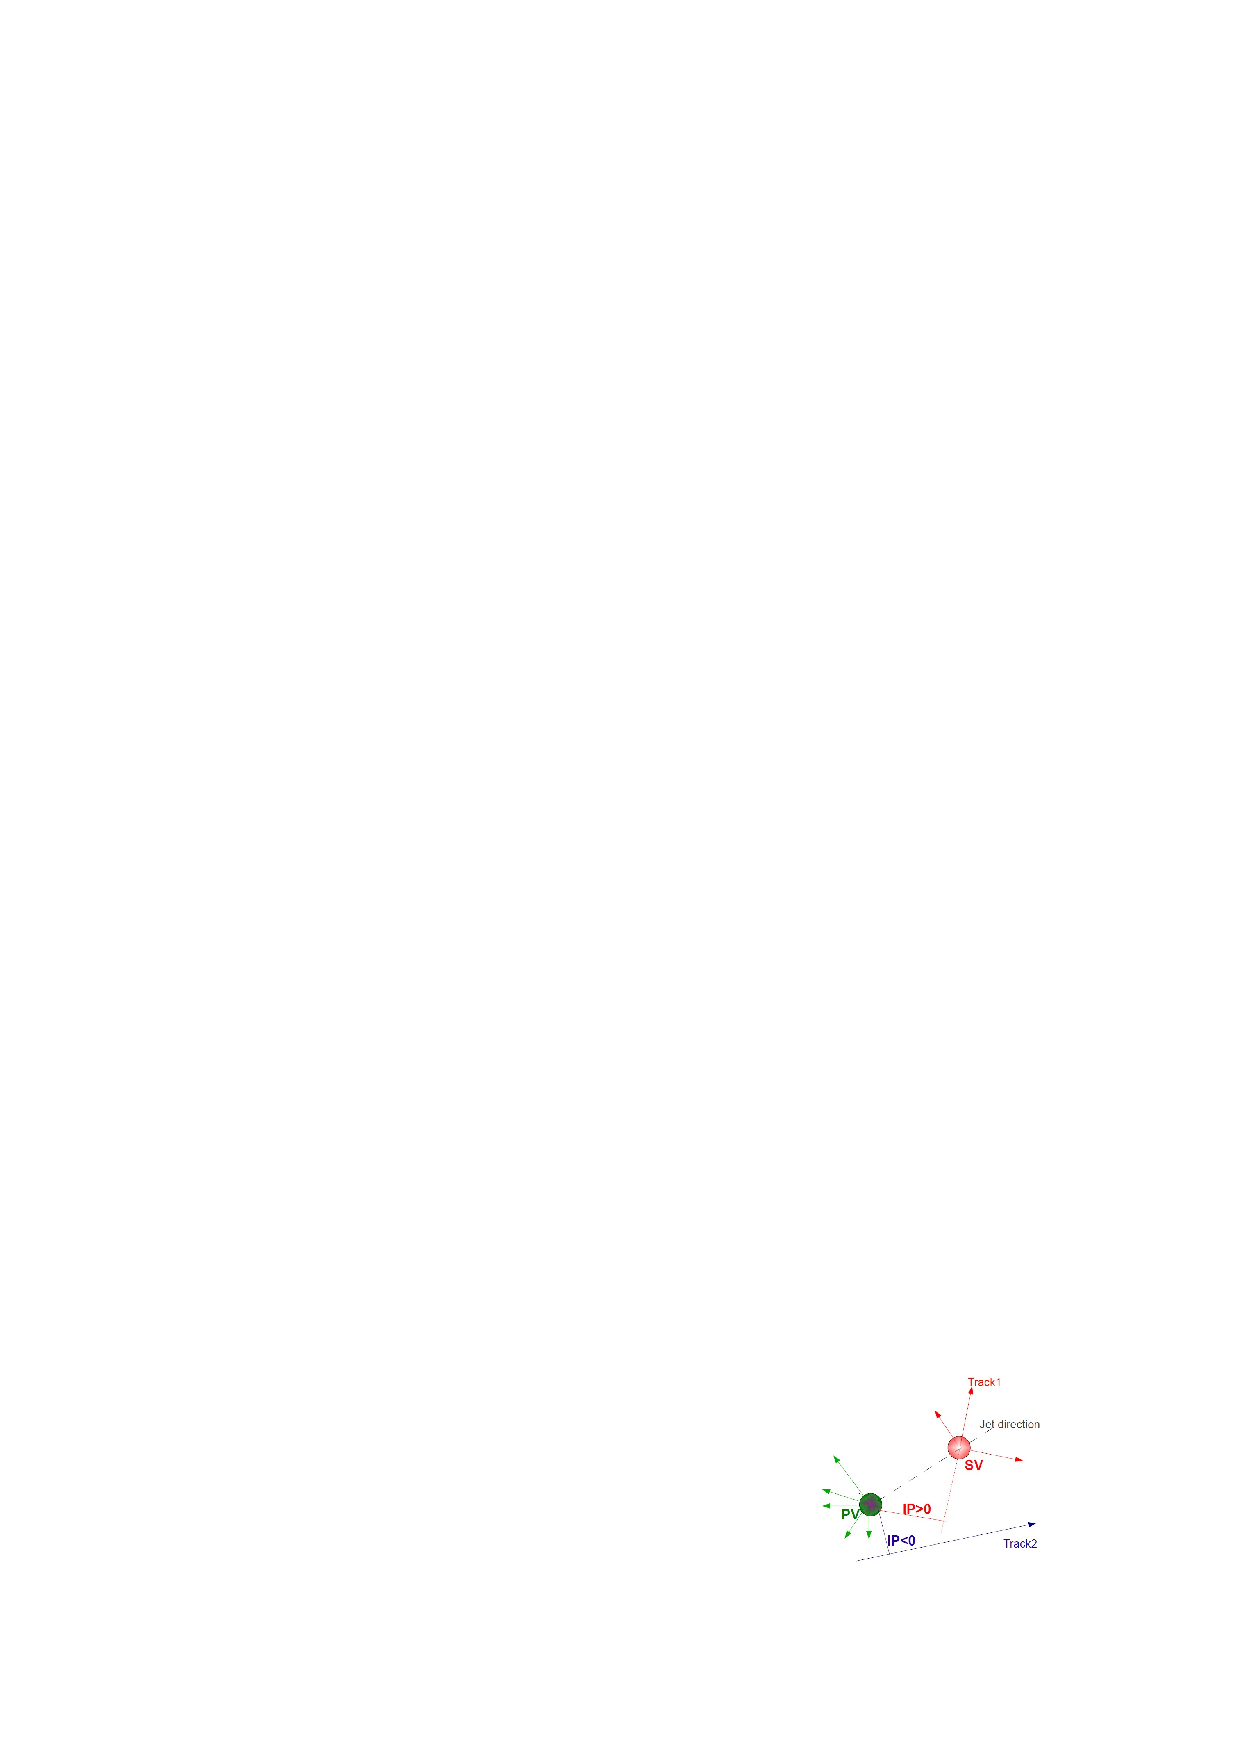
\includegraphics[width=0.50\linewidth]{Image/bCSV.pdf}
\caption{ Primary and secondary vertex with tracks and impact parameter. IP $> 0$ or $< 0$ if tracks
are upstream or downstream along the jet direction. This figure is taken from \cite{Ferro:2012tg}.} 
\label{fig:bCSV}
\end{figure}

\subsection{Track selection}
\label{ss:Track Selection}
The tracks are selected with the criteria listed in Table~\ref{tab:track_sel}.
These requirements ensure the tracks are closer to the PV and not coming from pileup vertices.
After track selection, the SV is reconstructed as described in the next section.
\begin{table}
  \caption{Track selection criteria. PCA stands for the point of closest approach.}
 \begin{center}
 \begin{tabular}{cc}\hline\hline
 Variable & Selection \\ \hline\hline
 $\pt$ associated with tracks & $>0.8$ \GeV \\
 number of hits associated with tracks in the tracker & $>8$ \\
 longitudinal component of IP & $< 0.3$~\unit{cm}\\
 distance between PCA of tracks from the PV and jet-axis & $<0.07$~\unit{cm}\\
 distance between PCA of tracks from the jet-axis and PV & $< 5$~\unit{cm}\\
 the displaced track should have & IP $>50$~\unit{$\mu$m} and $\frac{\rm {IP}}{\sigma_{\rm {IP}}}>1.2$\\\hline
 \end{tabular}
 \end{center}
 \label{tab:track_sel}
 \end{table}

\subsection{Reconstruction of secondary vertex}
For Run-I (proton-proton collisions at 8 \TeV), the {\em combined secondary vertex} (CSV) method used 
the adaptive vertex reconstruction algorithm~\cite{Waltenberger:1166320}, which is based on adaptive 
vertex fitter~\cite{Fruhwirth:1027031} to reconstruct the SV. On the other hand, in case of Run-II
(proton-proton collisions at 13 \TeV), the CSVv2 uses the inclusive vertex finder (IVF) 
algorithm~\cite{Khachatryan:2011wq} for the same purpose. The collection of selected tracks are used 
as inputs to the IVF. The displaced tracks are used as seed. The cluster of tracks is formed from 
seed track depending on the angles and distance between them. The adaptive vertex fitter is used to 
fit the clusters. The selection listed in Table~\ref{tab:sv_sel} are applied for the SV.
\begin{table}
  \caption{Secondary vertex selection criteria. $d_{\rm {PV, SV}}^{\rm {trans}}$ is the 2D flight
  distance or the distance between a primary and secondary vertex in the transverse plane.}
 \begin{center}
 \begin{tabular}{cc}\hline\hline
 Variable & selection \\ \hline\hline
     number of tracks associated with the SV & $>$ 2 \\
     $d_{\rm {PV, SV}}^{\rm {trans}}$ & $>$ 0.1~\unit{mm} \\
     $d_{\rm {PV, SV}}^{\rm {trans}}$ & $<$ 2.5~\unit{cm} \\
     mass associated with the SV & $<$ 6.5 \GeV\\
     $\Delta \rm R$ (jet axis, secondary flight direction) & $<$ 0.4\\ \hline
 \end{tabular}
 \end{center}
 \label{tab:sv_sel}
 \end{table}

\subsection{Multi-layer perceptron training}
Three types of discriminating variable, as shown below, are used in multi-layer perceptron training to identify the secondary vertex.
\begin{itemize}[leftmargin=*]
    \item category-I: jet with $N_{\rm {SV}} > 1$,
    \item category-II: jet with pseudo-vertex~\cite{CMS-PAS-BTV-15-001}, and
    \item category-III: jet with no SV or no pseudo-vertex.
\end{itemize}
The discriminating variables from the vertex-categories are combined using a likelihood ratio,
which gives the \PQb discriminator value.
The \PQb discriminator value for the \mujets and \ejets channel is shown in 
Figure~\ref{fig:pfCISV_lepBTag}. There are three official \PQb tagging working points: {\em loose}, {\em medium}, and {\em tight} with
\PQb tag efficiency [defined in Eq.~(\ref{eq:btag_eff})] 81\%, 63\%, and 41\%, respectively.
The corresponding probability of a light jet being misidentified as \PQb jet is 10\%, 1\%, and 0.1\%.
In this analysis, we use the medium working point \ie, \PQb discriminator $>$ 0.8484 for \PQb tagging.
The efficiency of all \PQb taggers for \PQb, \PQc, and light quarks are shown in Table~\ref{tab:bTagEff}. 
\begin{table}
\begin{center}
\caption{The efficiency of loose (L), medium (M), and tight (T) \PQb tag working points for different 
quark-flavor of jets \cite{Sirunyan:2017ezt}. These efficiencies are calculated from \ttbar events 
with jet \pt $>$ 20 \GeV.}
\begin{tabular}{cccccc}
\hline
\hline
Working point & $\epsilon^b$ (\%) & $\epsilon^c$ (\%) & $\epsilon^{udsg}$ (\%)& CSVv2 \\ \hline\hline
\PQb tagger L & 81 & 37 & 8.9 & $>$ 0.5426  \\
\PQb tagger M & 63 & 12 & 0.9 & $>$ 0.8484   \\
\PQb tagger T & 41 & 2.2& 0.1 & $>$ 0.9535   \\
\hline
\end{tabular}
\label{tab:bTagEff}
\end{center}
\end{table}

\begin{center}
\begin{figure}
\subfigure[]{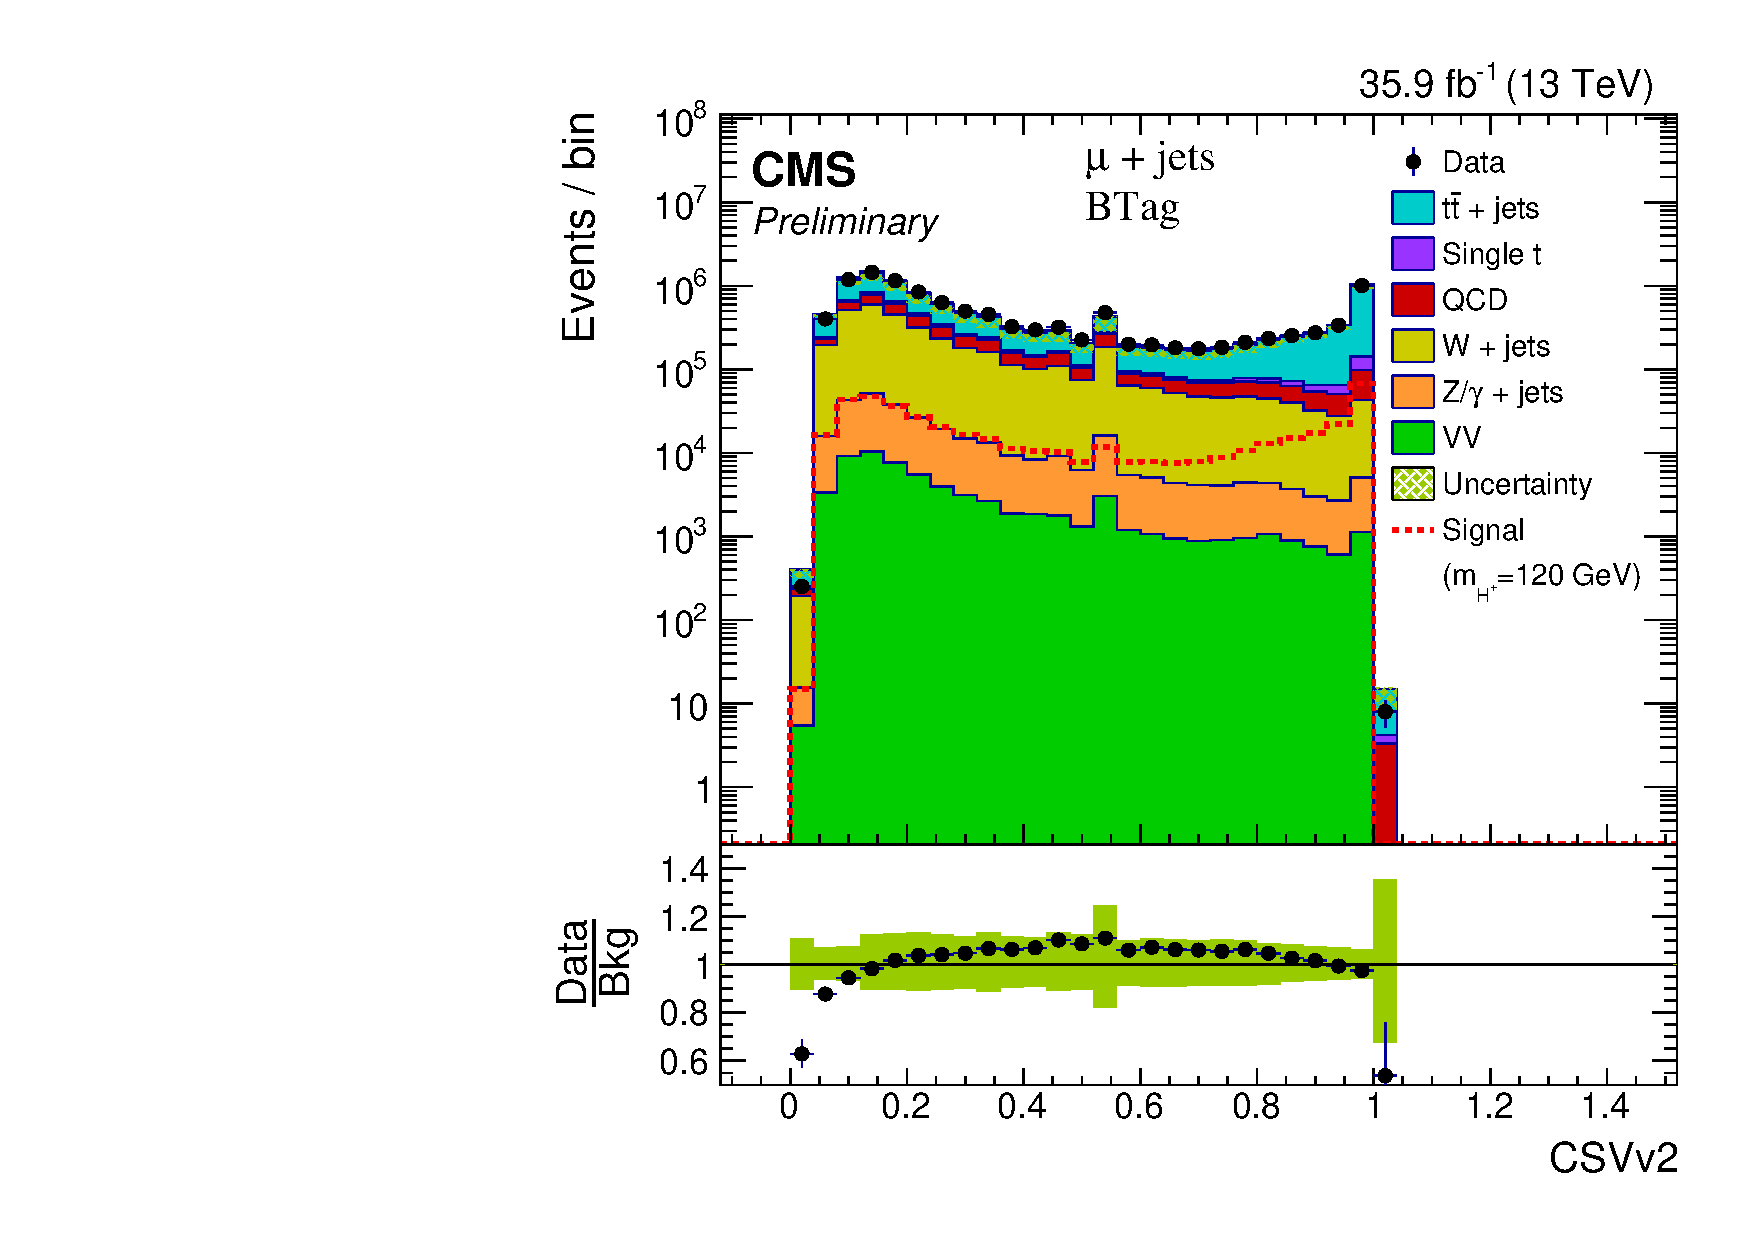
\includegraphics[width=0.50\linewidth]{Image/Muon/BTag/pfCISV_muBTag.pdf}}
\subfigure[]{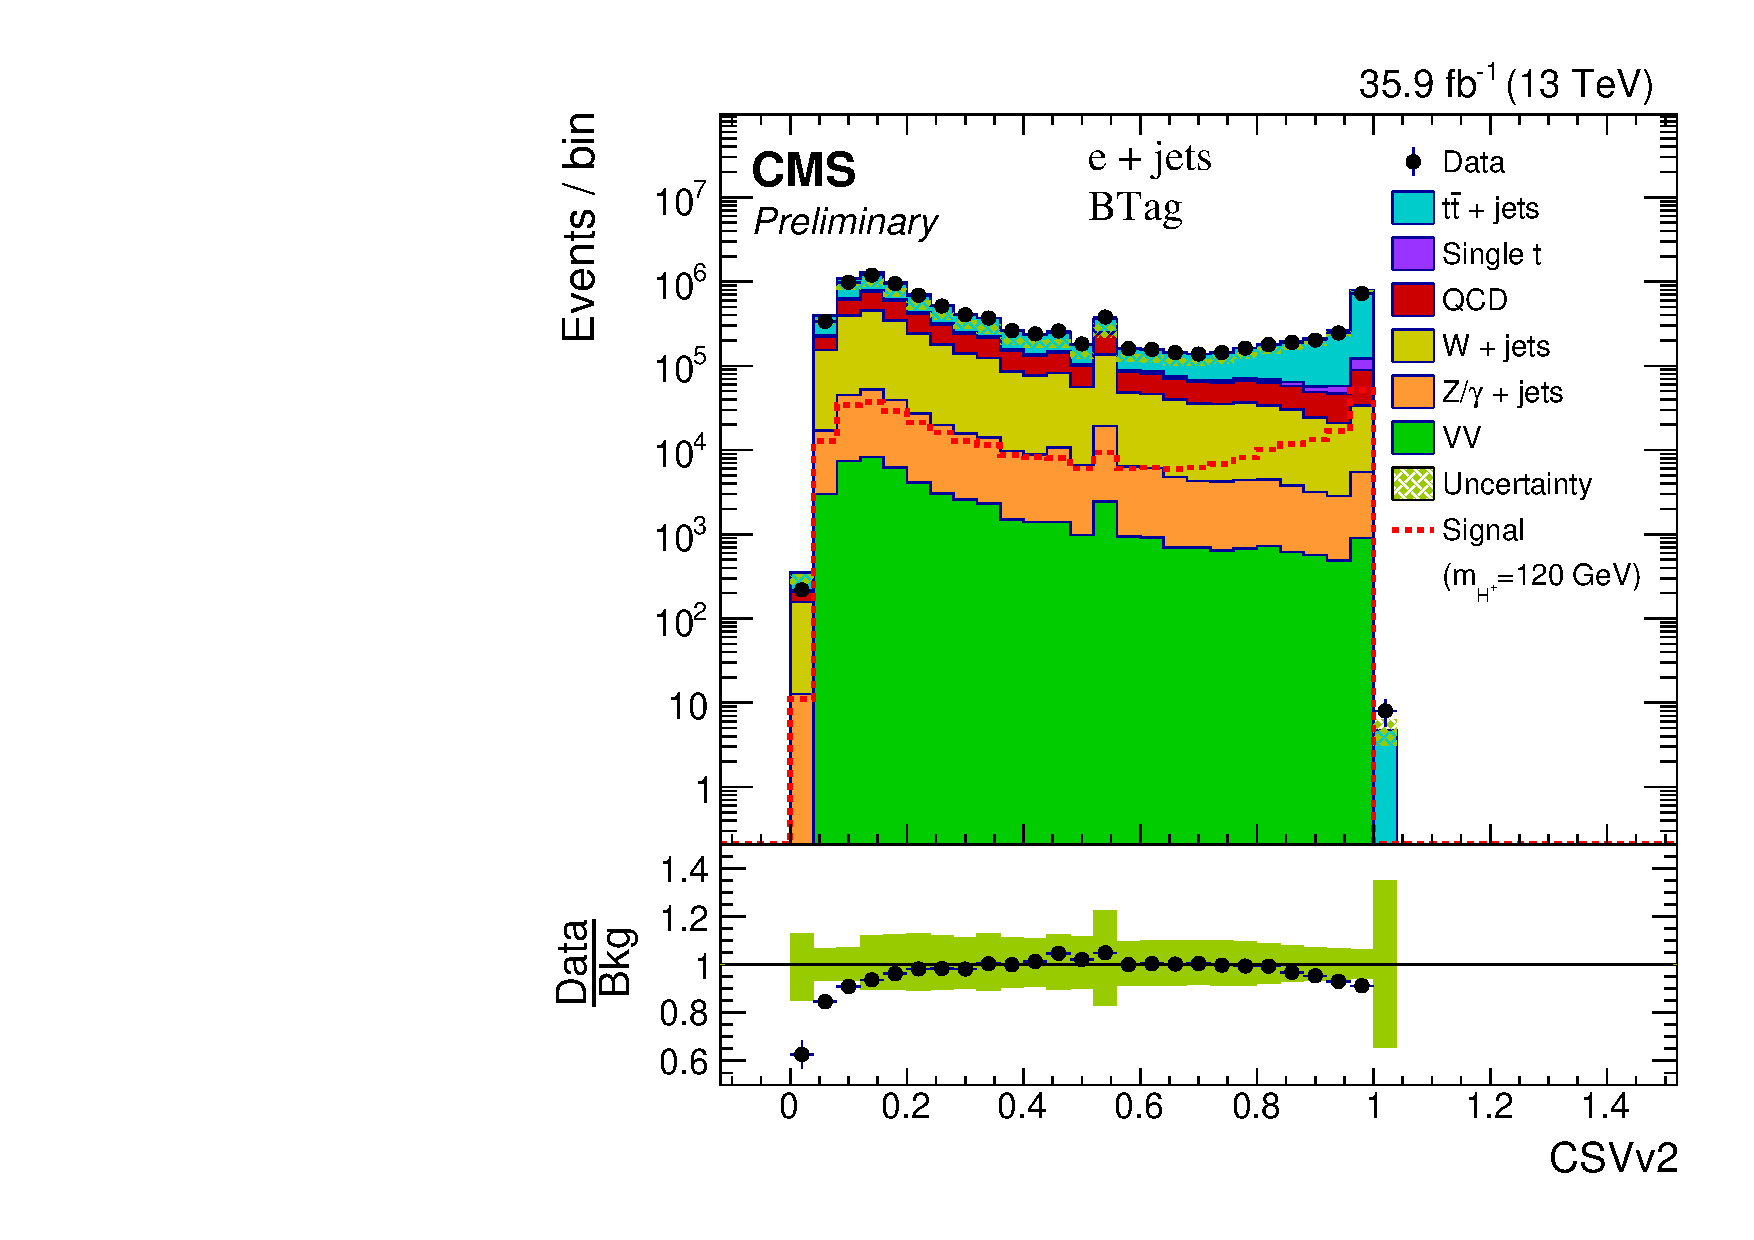
\includegraphics[width=0.50\linewidth]{Image/Electron/BTag/pfCISV_eleBTag.pdf}}
\caption{The \PQb discriminator distributions of all jets, after $N_{jets} \geq 4$ selection as described in Section~\ref{s:secEvtSel}, obtained using CSVv2 method for the \mujets and \ejets channel.}
\label{fig:pfCISV_lepBTag}
\end{figure}
\end{center}

